\documentclass[12pt,pdftex,a4paper,parskip=half]{scrbook} % Haupteinstellungen
\usepackage{ngerman} % Deutsche Sprachdatei
\usepackage[utf8]{inputenc} % Deutsche Umlaute
\usepackage[T1]{fontenc} % Schriftart
\usepackage{graphicx} % Grafiken einbinden
\usepackage{amsmath, amsthm, amssymb} % Mathematische Formeln
\usepackage{mathtools} % Mathematische Formeln
\usepackage{setspace} % Zeilenabstand
\usepackage{lmodern} % Vektorschriftart Modern
\usepackage{url} % Trennung URLs
\usepackage{acronym} % Abkürzungsverzeichnis
\usepackage{listings} % Code
\usepackage{booktabs} % Schöne Tabellen
\usepackage{tabularx} % Tabellen
\usepackage{scrhack} % Deprecated Methoden unterdrücken
\usepackage[backend=biber]{biblatex} % Gebraucht für BibStyle
\DeclareNameAlias{default}{last-first/first-last} % Erst Nachname im Literaturverzeichnis

\addbibresource{bib/Literatur.bib}

\newenvironment{itemize*}%
  {\begin{itemize}%
    \setlength{\itemsep}{2pt}%
    \setlength{\parskip}{2pt}}%
  {\end{itemize}}
  
\newenvironment{enumerate*}%
  {\begin{enumerate}%
    \setlength{\itemsep}{2pt}%
    \setlength{\parskip}{2pt}}%
  {\end{enumerate}}

\deffootnote{1em}{1em}{ %Einrueckung der Fussnoten wird korrigiert
	\textsuperscript{\thefootnotemark\ }
}

\lstset{%
	language=[LaTeX]TeX,     % Sprache des Quellcodes ist TeX
	stepnumber=1,            % Jede Zeile nummerieren.
	numbersep=5pt,           % 5pt Abstand zum Quellcode
	numberstyle=\tiny,       % Zeichengrösse 'tiny' für die Nummern.
	breaklines=true,         % Zeilen umbrechen wenn notwendig.
	breakautoindent=true,    % Nach dem Zeilenumbruch Zeile einrücken.
	postbreak=\space,        % Bei Leerzeichen umbrechen.
	tabsize=2,               % Tabulatorgrösse 2
	basicstyle=\ttfamily\footnotesize, % Nichtproportionale Schrift, klein für den Quellcode
	showspaces=false,        % Leerzeichen nicht anzeigen.
	showstringspaces=false,  % Leerzeichen auch in Strings ('') nicht anzeigen.
	extendedchars=true      % Alle Zeichen vom Latin1 Zeichensatz anzeigen.
} % Hintergrundfarbe des Quellcodes setzen.

%Trennung von Wörtern
\hyphenation{Such-er-geb-nis-se}
\hyphenation{Such-er-geb-nis-sen}
\hyphenation{Un-super-vised-Lear-ning}
\hyphenation{Lern-Al-go-rith-mus}

\pdfminorversion 6 % PDF-Version 1.6
\onehalfspacing % Zeilenabstand 1,5

\begin{document}
\pagestyle{plain} % Keine Kopfzeilen
\thispagestyle{plain}
\KOMAoptions{twoside = false}
\begin{titlepage}

\begin{center}
\LARGE{\textbf{Evaluierung, Analyse und Implementierung eines Machine Learning Verfahrens zur Verbesserung von fachlichen Entscheidungen}}\\[3ex]

\Large{\textbf{Bachelor-Thesis}}\\[1ex]
\Large{Fakultät Informatik}\\[4ex]


\includegraphics[width=9cm]{images/htwgknold.png}\\[5ex]

\Large{zur Erlangung des akademischen Grades}\\[1ex]
\Large{\textbf{Bachelor of Science}}\\[3ex]

\normalsize
\begin{tabular}{rl}\\
	vorgelegt von: & \quad Fabian Cotic\\[1.2ex]
	Studiengang: & \quad Wirtschaftsinformatik\\[1.2ex]
	Matrikelnummer: & \quad 288710\\[1.2ex]
	Erstgutachter: & \quad Prof. Dr. Christian Johner\\[1.2ex]
	Zweitgutachter: & \quad Dr. Bernd Michelberger\\[3ex]
\end{tabular}

\end{center}

\end{titlepage}

\KOMAoptions{twoside}

\advance\oddsidemargin by 0.5cm % Text verschieben
\advance\evensidemargin by -0.5cm % Text verschieben
 % Titelseite
\chapter*{Eidesstattliche Erklärung}

Hiermit versichere ich an Eides statt, dass ich die vorliegende Arbeit selbstständig verfasst und keine anderen als die angegebenen Quellen und Hilfsmittel benutzt habe, dass alle Stellen der Arbeit, die wörtlich oder sinngemäß aus anderen Quellen übernommen wurden, als solche kenntlich gemacht sind und dass die Arbeit in gleicher oder ähnlicher Form noch keiner Prüfungsbehörde vorgelegt wurde.
\vspace{1.5cm}

\rule{12cm}{0.2mm} \\
Ort, Datum, Unterschrift % Eidesstattliche Erklärung
\chapter*{Vorwort}

Die vorliegende Arbeit bildet den Abschluss meines Bachelor-Studiums der Fachrichtung Wirtschaftsinformatik an der HTWG Konstanz. Diese Arbeit ist im Zeitraum vom 01. Juni 2017 bis 31. August 2017 unter der Betreuung von Herrn Prof. Dr. Christian Johner und Dr. Bernd Michelberger entstanden. Das Thema der Arbeit entstand einerseits aus meinem persönlichen Interesse an Machine Learning, sowie steigenden Kundenanfragen bezüglich Machine Learning im Vertrieb der ACTICO GmbH. Aufgrund meiner vorigen Tätigkeiten im Unternehmen, kam mir die Ehre zuteil mein Thema selbst zu wählen und Mithilfe meines Betreuers Dr. Bernd Michelberger auszugestalten.

Johner ...

Bernd ... 

ACTICO ...

Korrekturleser ...

Zu Letzt möchte ich mich bei meinen Eltern bedanken, die mir während meines Studiums immer liebevoll mit Rat und Tat zur Seite standen und mich finanziell unterstützen um mir so mein Studium erst zu ermöglichen.   % Vorwort
\chapter*{Abstract}

Lorem ipsum dolor sit amet, consetetur sadipscing elitr, sed diam nonumy eirmod tempor invidunt ut labore et dolore magna aliquyam erat, sed diam voluptua. At vero eos et accusam et justo duo dolores et ea rebum. Stet clita kasd gubergren, no sea takimata sanctus est Lorem ipsum dolor sit amet. Lorem ipsum dolor sit amet, consetetur sadipscing elitr, sed diam nonumy eirmod tempor invidunt ut labore et dolore magna aliquyam erat, sed diam voluptua. At vero eos et accusam et justo duo dolores et ea rebum. Stet clita kasd gubergren, no sea takimata sanctus est Lorem ipsum dolor sit amet. Lorem ipsum dolor sit amet, consetetur sadipscing elitr, sed diam nonumy eirmod tempor invidunt ut labore et dolore magna aliquyam erat, sed diam voluptua. At vero eos et accusam et justo duo dolores et ea rebum. Stet clita kasd gubergren, no sea takimata sanctus est Lorem ipsum dolor sit amet. Duis autem vel eum iriure dolor in hendrerit in vulputate velit esse molestie consequat, vel illum dolore eu feugiat nulla facilisis at vero eros et accumsan et iusto odio dignissim qui blandit praesent luptatum zzril delenit augue duis dolore te feugait nulla facilisi. Lorem ipsum dolor sit amet, consectetuer adipiscing elit, sed diam nonummy nibh euismod tincidunt ut laoreet dolore magna aliquam erat volutpat.  % Abstract\tableofcontents % Inhaltsverzeichnis
\clearpage % Neue Seite
\addchap{Abkürzungsverzeichnis}
\begin{acronym}
    \acro{BKM}{Business Knowledge Model}
	\acro{BPMN}{Business Process Model and Notation}
	\acro{CORBA}{Common Object Request Broker Architecture}
	\acro{DM}{Decision Management}
	\acro{DMN}{Decision Model and Notation}
	\acro{DMS}{Decision Management Systems}
	\acro{DS}{Decision Service}
	\acro{DRD}{Decision Requirements Diagramm}
	\acro{OMG}{Object Management Group}
	\acro{ML}{Machine Learning}
	\acro{UML}{Unified Modeling Language}
\end{acronym} % Abkürzungsverzeichnis
\cleardoublepage % Neue Seite
\addcontentsline{toc}{chapter}{Abbildungsverzeichnis} % Überschrift Abbildungsverzeichnis
\listoffigures % Abbildungsverzeichnis
\cleardoublepage % Neue Seite
\addcontentsline{toc}{chapter}{Tabellenverzeichnis} % Überschrift Tabellenverzeichnis
\listoftables % Tabellenverzeichnis
\tableofcontents % Inhaltsverzeichnis
\chapter{Motivation}
\label{ch:Motivation1}
 
Unternehmen treffen unzählige Entscheidungen jeden Tag. Wertschöpfende Entscheidungen tragen, wie ihr Name schon sagt, zur Wertschöpfung bei und beeinflussen somit unmittelbar den wirtschaftlichen Erfolg eines Unternehmens. Eine Bank beispielsweise muss einen Kreditnehmer auf dessen Fähigkeit, Raten zurückzahlen zu können, prüfen. Somit soll sichergestellt werden, dass die Bank den Betrag des Kredites sowie auch die ihr zustehenden Zinsen zurückbekommt. Dadurch steht und fällt der Erfolg einer Bank mit den Krediten, die sie vergibt \cite[vgl. S. 1]{AF04}. Prominentestes Beispiel hierfür ist die ehemalige US-amerikanische Investmentbank Lehmann Brothers, die im Zuge der Finanzkrise 2008 Insolvenz anmelden musste \cite[vgl. S. 3]{WN09}. Boomende Immobilien-Preise resultierten in höheren Sicherheiten von Privathaushalten, wodurch auch Kredite an Darlehnsnehmer mit geringer Bonität vergeben wurden (Subprime-Kredit) \cite[vgl. S. 82-83]{MB09}. Nach dem Platzen der Immobilienblase kam es zu Zahlungsausfällen und -störungen im US-amerikanischen Hypothekenmarkt \cite[vgl. S. 6 ff.]{RK10}, was erst in einem Finanzcrash und dann in einer Weltwirtschaftskrise resultierte \cite[vgl. S. 109]{LG09}.

Etwa im Juni 2009 waren die schlimmsten Auswirkungen der Finanzkrise überstanden, die amerikanische Wirtschaft begang wieder zu wachsen \cite[vgl. S. 21]{HR10} und Banken vergaben fleißig Kredite. Heutzutage werben Banken mit Kreditentscheidungen innerhalb von wenigen Sekunden. Das Ausfüllen eines Formulars ist ausreichend, um wenige Sekunden später eine Kreditentscheidung zu erhalten. Die Prüfung der Bonität geschieht automatisiert im Hintergrund durch eine zuvor definierte Entscheidungslogik. Die Entscheidungslogik wird von Fach-Experten erstellt, wobei die Fach-Experten im Wesentlichen zwei essentielle Dinge beachten:
 
\begin{enumerate*}
\item Verhinderung der Vergabe von Krediten an Personen, die diese 
nicht zurückzahlen können (''default rate'') 
\item Verhinderung der Nicht-Vergabe von Krediten an Personen, die eigentlich in der Lage 
sind, diese zurück zuzahlen, wodurch Einnahmen an Konkurrenten 
verloren gehen (''acceptance rate'') \end{enumerate*}

Banken sind somit angehalten eine gute Balance zwischen Sicherheit und Gewinn zu finden. Dazu muss die fachliche Entscheidungslogik drohende Zahlungsausfälle so genau wie möglich vorhersagen. Studien wie \cite[]{IM17} zeigen, dass sieben Prozent der vergebenen Kredite im Euroraum mehr als 90 Tage im Zahlungsverzug sind. Das entspricht einem Volumen von einer Billionen Euro. Bei einem Zahlungsverzug von über 90 Tagen wird generell davon ausgegangen, dass ein Kredit nicht mehr in voller Höhe zurückgezahlt wird und somit zu einem Verlust-Geschäft führt \cite[vgl. S. 8]{BF05}. Könnte man die Entscheidungslogiken bei den Banken dahingehend optimieren, ein Prozent weniger ''faule'' Kredite zu vergeben, könnten große Summen eingespart werden, die sonst im Zuge einer Banken-Rettung dem Steuerzahler auferlegt werden.        

\section{Problemstellung}
\label{sec:Problemstellung1}

Das Einsparen der genannten Summen wäre erstrebenswert, allerdings gibt es unzählige Gründe, die den Finanzcrash ab 2007 verschuldet haben. Als Hauptgrund wird in der Literatur die umfangreiche Vergabe von Subprime-Krediten genannt \cite[]{MB09, WN09}. Bei der Vergabe dieser Kredite wurde das Risiko nicht korrekt identifiziert \cite[vgl. S. 3]{WN09}, was zu unzähligen falschen fachlichen Entscheidungen führte. Daraus abgeleitet ergibt sich die Problemstellung dieser Arbeit, dass zu viele fachliche Entscheidungen falsch getroffen werden. Die Gründe hierfür werden nachfolgenden beschrieben und in Abbildung \ref{fig:Gruende} zusammengefasst.   

\begin{figure}[ht] 
\centering
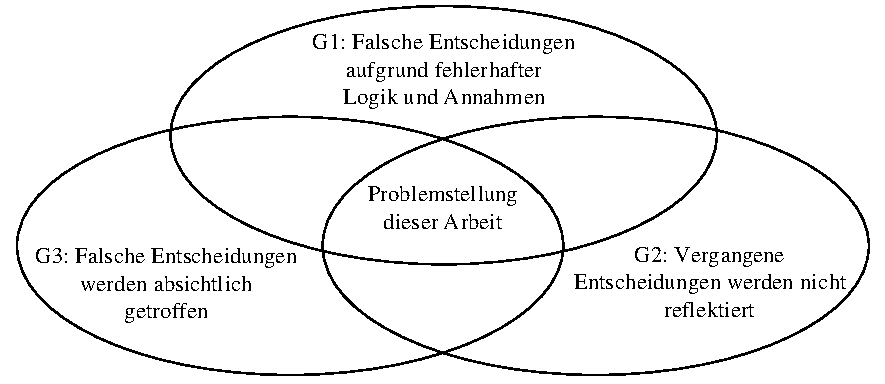
\includegraphics{images/gruende.pdf}
\caption{Gründe für falsch getroffene fachliche Entscheidungen.}
\label{fig:Gruende}
\end{figure}

Ein Grund für die vielen falschen Entscheidungen, sind fehlerhafte Entscheidungslogiken und falsche Annahmen (Grund G1 - siehe Abbildung \ref{fig:Gruende}). Bei der Vergabe der Kredite wurden die Entscheidungen verfälscht, da die Entscheidungslogiken mit Eingabe-Daten befüllt wurden, die nicht der Realität entsprachen. Durch die unrealistisch hohen Immobilien-Preise, waren die Kredite mit Immobilien gesichert, die real weitaus weniger wert waren \cite[]{HR11}. Die Kredite wurden dementsprechend auf Basis von nicht vorhandenen Sicherheiten berechnet.

Ein weiterer Grund ist, dass vergangene Entscheidungen nicht mehr reflektiert wurden. (Grund G2 - siehe Abbildung \ref{fig:Gruende}). Die Kredite wurden gebündelt unter den Banken weiterverkauft \cite[vgl. S. 2]{WN09}, ein Verlust-Risiko bestand somit nur für die kurze Zeit, in der ein Kredit-Bündel noch nicht weiterverkauft wurde. Saunders et al. sagen ''The underwriters [...] had little incentive to screen and monitor the activities of borrowers for whom they originated loans'' \cite[]{SA10}. Nach der ursprünglichen Vergabe des Kredites, wurden also keine weitere Aktivitäten unternommen, um die damaligen Kredit-Entscheidungen weiterhin zu prüfen oder zu überwachen. Ein Kontrollverlust der Situation war nur eine Frage der Zeit.            

Im Falle der Finanzkrise waren allerdings nicht nur fehlerhafte Entscheidungslogik, falsche Annahmen und mangelnde Reflektion schuld am Zusammenbrauch der Finanzmärkte. Absichtlich falsch getroffene Entscheidungen sind ebenso als Ursache der vielen falsch getroffenen Entscheidungen anzuführen (Grund G3 - siehe Abbildung \ref{fig:Gruende}). In einer Pressemitteilung des Vorstandes der US-Notenbank, wurden Bonus-Zahlungen an Bank-Mitarbeiter als weiterer Grund der Finanzkrise aufgezählt: ''Flaws in incentive compensation practices were one of many factors contributing to the financial crisis. Inappropriate bonus or other compensation practices can incent senior executives or lower level employees, such as traders or mortgage officers, to take imprudent risks that significantly and adversely affect the firm'' \cite[]{BG09}. Mitarbeiter übertraten bewusst Risiken, nutzten mangelnde Regulationen zu ihrem Vorteil und ließen keine Möglichkeit aus ihren Gewinn auf Kosten von Stabilität und Sicherheit zu maximieren. 

Zusammenfassend soll Abbildung \ref{fig:Gruende} nochmals die Gründe aufzeigen die verantwortlich sind, dass zu viele falsche fachliche Entscheidungen getroffen werden.

\section{Zielsetzung}
\label{sec:Zielsetzung1}

Das übergeordnete Ziel ist die in \ref{sec:Problemstellung1} genannte Problemstellung, dass zu viele falsche fachliche Entscheidungen getroffen werden, zu verbessern, indem man die Anzahl falscher fachlichen Entscheidungen reduziert. Diese Arbeit soll hierzu ein Machine Learning (ML) Verfahren evaluieren, analysieren und implementieren, um fachliche Entscheidungen zu verbessern. Aus dieser Zielsetzung können die folgenden Teilziele abgeleitet werden. 

Das \textit{erste Teilziel} ist das Erstellen und die kontinuierliche Optimierung von Modellen, anhand von vergangen fachlichen Entscheidungen und deren Korrektheit. Dazu soll im ersten Schritt ein ML-Verfahren implementiert werden, das Modelle aus den Daten vergangener Entscheidungen generiert. Die Datensätze dieser Entscheidungen werden um ein weiteres Attribut ergänzt, die Performance. Die Performance beschreibt den Fall, der sich in der realen Welt als der richtige erwiesen hat. Bei der Kredit-Entscheidungslogik beispielsweise, wäre die Performance ob ein Kunde seinen Kredit zurückgezahlt hat oder nicht. Das ML-Verfahren, soll die Kombination von Input-Daten und Performance auf Gesetzmäßigkeiten prüfen und diese anschließend als Modell zur Verfügung stellen. Ein Modell beschreibt den Output eines ML-Verfahrens und bietet zwei fundamentale Mechanismen. Erstens soll das Modell in der Lage sein, weiter optimiert werden zu können (''lernen''), zweitens soll für einen gegebenen Input-Datensatz ein dazugehörender Output vorhergesagt werden (''evaluieren''). 

Das \textit{zweite Teilziel} besteht darin Modelle heranzuziehen, um Entscheidungslogiken so zu verbessern, dass zukünftige fachliche Entscheidungen korrekter getroffen werden. Das erlernte Modell wird  dazu verwendet, mehrere Datensätze zu evaluieren und den Ausgang deren Entscheidungen vorherzusagen. Die daraus resultierenden Ergebnisse sollen dann in den Entscheidungsfindungsprozess mit einfließen und somit zu mehr richtig getroffenen Entscheidungen verhelfen. 

Auf Basis dieser Teilziele ergeben sich eine Reihe von Forschungsfragen: 

\begin{itemize*}
\item \textbf{Forschungsfrage 1:} Können ML-Verfahren verwendet werden, um fachliche Entscheidungen zu verbessern? 

- Was gibt es für einsetzbare ML-Verfahren?

- Welche ML Verfahren eignen sich am besten?

\item \textbf{Forschungsfrage 2:} Wie können einsetzbare ML-Verfahren anhand eines fachlichen Anwendungsfall angewendet werden? 

- Welche Anwendungsfälle eignen sich hierzu?

- Was für Ergebnisse liefern diese? 

- Wie können die Ergebnisse interpretiert werden?

\item \textbf{Forschungsfrage 3:} Wie kann die Funktionsweise des ML-Verfahrens in ein Modell überführt werden, ohne dass dabei Performance-Daten offen gelegt oder zur Verfügung gestellt werden müssen?

\item \textbf{Forschungsfrage 4:} Wie kann sichergestellt werden, dass die fachliche Entscheidung verbessert werden können?
\end{itemize*}


Die vier Forschungsfragen werden in Tabelle /ref{tab:chapters} 1.2 zu einem oder mehreren Kapiteln dieser Thesis zu geordnet. 

\begin{table}[htb]
\centering
\small
\begin{tabular}{lccccccc}
\toprule
\# & Kap. 1 & Kap. 2 & Kap. 3 & Kap. 4 & Kap. 5 & Kap. 6 & Kap. 7\\
\toprule
Forschungsfrage 1 &  & $\times$ & & &$\times$& &\\\midrule
Forschungsfrage 2 &  &$\times$& $\times$ & $\times$ & & &\\\midrule
Forschungsfrage 3 &  & &  $\times$ & $\times$& & &\\\midrule
Forschungsfrage 4 &  &  $\times$& $\times$ &  $\times$&$\times$  & &\\\bottomrule
\end{tabular}
\caption{Forschungsfragen entlang der Kapitel.}
\label{tab:chapters}
\end{table}

\section{Abgrenzung}
\label{sec:Abgrenzung1}

Einhergehend mit den zu beantwortenden Forschungsfragen findet auch folgende Abgrenzung statt: Es ist kein Ziel dieser Arbeit, einen eigenen ML-Algorithmus zu entwickeln. Die Entwicklung eines eigenen Algorithmus ist nicht notwendig, da in der Literatur und Praxis schon vielversprechende Algorithmen entwickelt worden sind. Vielmehr sollen bereits bestehende Algorithmen und Lösungen, die sich in der Praxis als erfolgreich bewiesen haben, intelligent verknüpft werden, um fachliche Entscheidungen zu verbessern.  Ziel dieser Arbeit ist ausschließlich das Verbessern von automatisierbaren Entscheidungen. Entscheidungen können operativer und strategischer Natur sein, wobei sich nur operative Entscheidungen zur Automatisierung eignen. Tabelle \ref{tab:decisions} \cite[vgl. S. 9]{FT12} soll die Unterscheidung zwischen strategischen und operativen Entscheidungen verdeutlichen.  

\begin{table}[htb]
\centering
\small
\begin{tabular}{lcccc}
\toprule
Level of Decision &  Individual Value & Frequency & Data Required & Knowledge Required\\
\toprule
Strategic & High & Low & High & High\\\midrule
Operational & Low & High & Low & Low\\\bottomrule
\end{tabular}
\caption{Unterscheidung strategische und operative Entscheidungen.}
\label{tab:decisions}
\end{table}  
    
\section{Aufbau der Arbeit}
\label{sec:Aufbau_der_Arbeit1}

Die vorliegende Bachelorarbeit besteht aus sieben Kapiteln, die sich nochmals in drei Teile (Teil I - Teil III) aufgliedern (siehe Abbildung \ref{fig:Aufbau}).

\begin{figure}[ht]
\centering
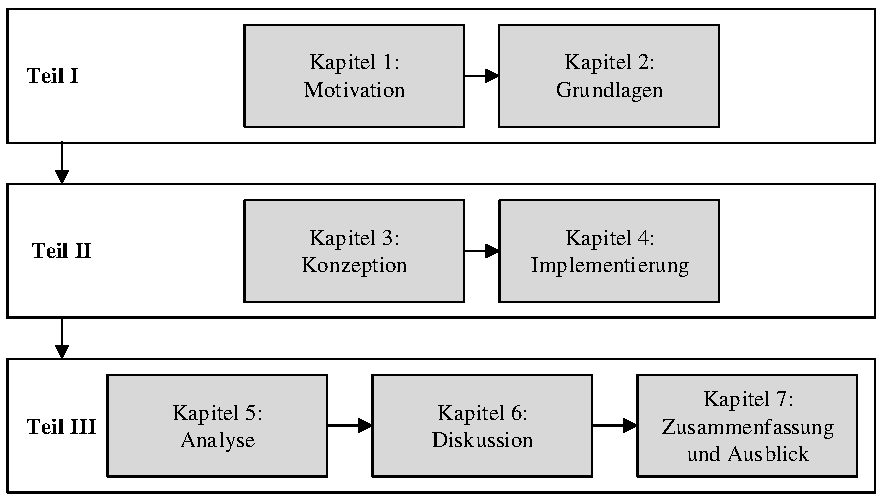
\includegraphics{images/Aufbau.pdf}
\caption{Aufbau der Arbeit.}
\label{fig:Aufbau}
\end{figure}

\textbf{Teil 1} umfasst neben diesem einleitenden Kapitel die theoretischen Grundlagen, die für das weitere Verständnis benötigt werden. Kapitel \ref{sec:Decision_Management2} erläutert wie Entscheidungen abgebildet werden können, anschließend werden die Grundlagen von ML vermittelt (Kapitel \ref{sec:Machine_Learning2}), um im Anschluss verwendbare Technologien für Decison Management und ML zu identifizieren (Kapitel \ref{sec:Technologien2}).  

\textbf{Teil 2} befasst sich mit der Konzeption des Prototypen (Kapitel 3), sowie dessen Implementierung (Kapitel 4) und stellt damit den Hauptteil dieser Arbeit dar. Hierzu sollen zuerst Anwendungsfälle genannt werden (Kapitel 3.1), wovon anschließend Anforderungen abgeleitet und spezifiziert werden (Kapitel 3.2). Mit dem Abschluss der Konzeption, wird die Implementierung des Prototypen beschrieben. Hierzu wird zunächst die Implementierung des Datenschemas dargelegt (Kapitel 4.1), bevor die Implementierung der zu verbessernden Entscheidungslogik (Kapitel 4.2) erläutert wird. Aufbauend auf der Entwicklung des Datenschemas und der Entscheidungslogik, kann das ML-Verfahren implementiert (Kapitel 4.3) und optimiert werden (Kapitel 4.4).        

\textbf{Teil 3} bildet den Schlussteil der Arbeit und umfasst die Analyse (Kapitel 5), die Diskussion (Kapitel 6) und die Zusammenfassung inklusive eines Ausblicks (Kapitel 7).


\chapter{Grundlagen}
\label{ch:Grundlagen2}

Dieses Kapitel rundet den ersten Teil dieser Arbeit ab, indem die theoretischen Grundlagen beschrieben werden, die für das weitere Verständnis dieser Arbeit erforderlich sind. Hierzu zählen Decision Management (DM) und Machine Learning. 

\section{Decision Management}
\label{sec:Decision_Management2}

Unternehmen treffen unzählige Entscheidungen jeden Tag, um so wichtiger ist ein zentraler Ort an dem Entscheidungen verwaltet werden können. \emph{Decision Management} (DM) adressiert die Verwaltung von automatisierten Entscheidungen, über den kompletten Lebenszyklus von Entscheidungen hinweg. Dieser beinhaltet die Modellierung, Ausführung, Überwachung und die Optimierung, mit dem Ziel fachliche Entscheidungen zu verbessern, indem der Lebenszyklus kontinuierlich durchlaufen wird. Abbildung \ref{fig:lifecycle} zeigt die einzelnen Phasen des Entscheidungs-Lebenszyklus, deren Erläuterung folgt im Anschluss.  

\begin{figure}[ht]
\centering
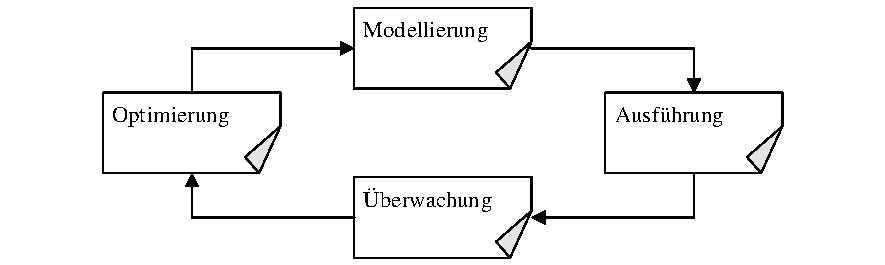
\includegraphics{images/lifecycle.pdf}
\caption{Der DMN Lebenszyklus.}
\label{fig:lifecycle}
\end{figure}

\textbf{Modellierung}. Zur Modellierung von Entscheidungen wurde 2015 der Standard Decison Model and Notation (DMN), von der Objekt Management Group veröffentlicht. Rücker nennt die Schaffung eines Notationsstandards für Entscheidungen, der für Fach- und IT-Anwender gleichermaßen verständlich ist, als oberstes Ziel von DMN \cite[vgl. S. 40]{BR16}.  Die offizielle DMN-Spezifikation nennt die Erfüllung der folgenden drei Anforderungen, als Ziel von DMN \cite[vgl. S. 18 ff.]{OM16}: 

\begin{enumerate*}
\item Modellierung von Entscheidungen, die von Menschen getroffen werden
\item Modellierung von Entscheidungen, die automatisiert getroffen werden 
\item Implementierung von automatisierten Entscheidungen    
\end{enumerate*}

Zur Umsetzung der genannten Anforderungen, definiert DMN zwei verschiedene Ebenen: Die Entscheidungsanforderungsebene (deskriptiv) und die Entscheidungslogikebene (präskriptiv), beide zusammen bilden das \emph{Decision Model}. Auf der Entscheidungsanforderungsebene, werden die Anforderungen die eine Entscheidung benötigt in einem Decision Requirements Diagrams (DRD) modelliert. Ein DRD, besteht aus Entscheidungen, Input-Daten, Business Knowledge Models und Knowledge Sources. Abbildung \ref{fig:drd} \cite[vgl. S. 21]{OM16} zeigt die genannten Elemente eines beispielhaften DRD und deren Notation.     

\begin{figure}[ht]
\centering
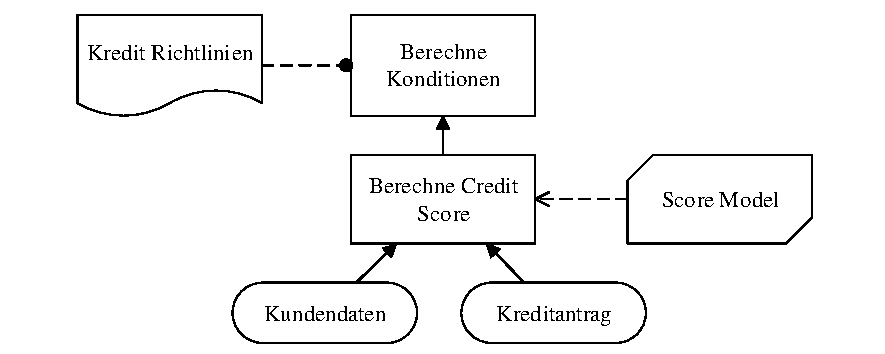
\includegraphics{images/drd.pdf}
\caption{Ein beispielhaftes Decision Requirements Diagram.}
\label{fig:drd}
\end{figure}

\textbf{Input-Data-Element:} Ein Input-Data-Element beschreibt Informationen, die als Eingabe für eine oder mehrere Entscheidungen dient \cite[vgl. S. 30]{OM16}. Abbildung \ref{fig:drd} zeigt die beiden Input-Daten-Elemente Kundendaten und Kreditantrag. 

\textbf{Business-Knowledge-Model-Element:} Ein Business Knowledge Model beschreibt eine Funktion die Fachwissen kapselt, beispielsweise als Geschäftsregel, Entscheidungstabelle, oder als analytisches Model \cite[vgl. S. 30]{OM16}. In Abbildung \ref{fig:drd} kapselt das Score Model das Fachwissen zur Berechnung des Credit Score.

\textbf{Decision-Element:} Ein Decision-Element beschreibt eine Entscheidung. Sie bestimmt einen Output, anhand verschiedener Inputdaten, mithilfe von Entscheidungslogik \cite[vgl. S. 20]{OM16}. In Abbildung \ref{fig:drd} wird der Credit Score mittels der Inputdaten Kreditantrag und Kundendaten berechnet.

\textbf{Knowledge-Source-Element:} Eine Knowledge-Source beschreibt die Quelle einer Entscheidung oder eines Business Knowledge Models. Das kann beispielsweise ein Dokument, oder auch ein Fach-Experte sein \cite[vgl. S. 18]{OM16}. Im vorliegenden Beispiel werden die Konditionen des Kredites durch die Vorgaben der Kredit Richtlinien berechnet.

Nun gilt es sich der Entscheidungslogik-Ebene zu widmen, die insbesondere für die automatisierte Ausführung von Entscheidungen essentiell ist \cite[vgl. S. 18]{OM16}. DMN erlaubt den Import von existierenden Entscheidungslogik-Standards. Der wohl wichtigste Entscheidungslogik-Standard im Umfeld von DMN ist die Entscheidungstabelle. Taylor definiert Entscheidungstabellen als: ''a look-up table where each cell represents an executable business rule. The conditions of the rule are columns or rows in the decision table and the intersection of the rows and columns shows the consequence of the rule'' \cite[S. 132]{JT11}. 

\begin{figure}[ht]
\centering
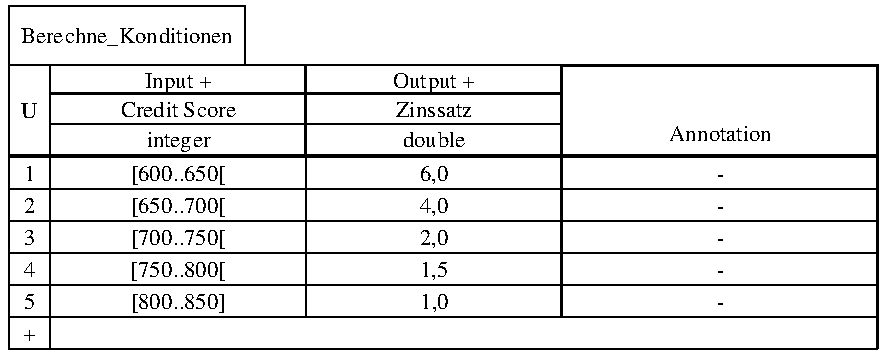
\includegraphics{images/decisiontable.pdf}
\caption{Beispiel einer Entscheidungstabelle zur Berechnung des Zinses.}
\label{fig:decisiontable}
\end{figure} 


Abbildung \ref{fig:decisiontable} zeigt eine Entscheidungstabelle zur Bestimmung des Zinses, anhand eines Credit Scores. Wäre der Credit Score beispielsweise 632, würde die erste Zeile der Entscheidungstabelle zutreffen und der Zins 6 Prozent betragen. Durch die Erläuterung von DRD und Entscheidungstabellen, sind alle relevanten Aspekte zur Modellierung von Entscheidungen geklärt. 

\textbf{Ausführung}. Um Decision Models ausführen zu können, müssen diese in einem geeigneten DMN-Tool modelliert werden. Zur vollständigen Automatisierung der Entscheidungen, muss die Entscheidungslogik in der Lage sein, für jeden möglichen Satz von Input-Daten einen
Entscheidungsausgang bestimmen zu können. DMN-Tools bieten Bibliotheken an, mit deren Hilfe eine Decision Engine implementiert werden kann. ''Eine Decision Engine ist ein Stück Software, das eine zustandslose Schnittstelle bereitstellt, um Entscheidungen auf Basis der in DMN definierten Entscheidungslogik zu fällen'' \cite[S. 41]{BR16}. Nach der Inbetriebnahme der Decision Engine bedürfen die getroffenen Entscheidungen der Überwachung.

\textbf{Überwachung}. Taylor nennt vier Faktoren, die kontrolliert werden sollen und dazu führen das Entscheidungen verbessert werden müssen \cite[vgl. S. 158]{JT11}:

\begin{enumerate*}
\item Änderungen an wirtschaftlichen Zielsetzungen
\item Neue Regularien oder Richtlinien
\item Änderungen an zugrundeliegenden Datenschemata  
\item Gesamt Performance der Entscheidungen\end{enumerate*}   

Auf die ersten drei Faktoren muss bei deren Eintritt reagiert werden, wohingegen der vierte Faktor einer ständigen Untersuchung bedarf. Proaktive-Änderungen an Entscheidungslogiken bieten Möglichkeiten, die Effektivität unserer Entscheidungen zu steigern, um somit unseren wirtschaftlichen Zielsetzungen näher zukommen. Wie effektiv oder gut eine Entscheidung ist definiert Taylor folgendermaßen:''The goals and key performance indicators or metrics of your business set a context that defines what a good or an effective decision looks like. The data you have collected over time gives you insight into what works and what doesn't, which is reflected in your current decision-making approach.'' \cite[vgl. S. 159]{JT11}. Die Analyse der Daten vergangener Entscheidungen ist unerlässlich um Proaktiv Entscheidungslogiken zu verbessern. Um eine effektive Überwachung und Verbesserung zu ermöglichen, müssen umfangreiche Datenmengen über die Effektivität unsere Entscheidungen gesammelt werden. Dazu zählen \cite[vgl. S. 164]{JT11}:

\begin{enumerate*}
\item \textbf{Decision-Service-Ausführungs-Daten:} Hierzu zählen alle Daten die während der Ausführung einer Entscheidung erhoben werden können. Beispielsweise IDs, Zeitstempel, Eingabe-Daten, Ausgabedaten, die Quelle des Aufrufs, oder kontextbezogene Daten die während der Ausführung generiert wurden.   
\item \textbf{Decision-Service-Antwort-Daten:} Meistens ergibt sich aus einer Entscheidung heraus eine Konsequez für den Empfänger der Entscheidung. Um nochmals das Beispiel der Online-Kredit-Bewerbung aufzugreifen, nachdem der Kreditantrag von unserem DS evaluiert und das Ergebnis zurückgeliefert wurde, kann die Reaktion des Empfängers gespeichert werden. Der Empfänger kann das zurückgelieferte Kreditangebot ablehnen, zustimmen, mehr Informationen verlangen oder für später abspeichern. Gelingt es die Reaktion des Empfängers, mit der Entscheidung zur späteren Analyse abzuspeichern, können daraus wertvolle Rückschlüsse über die Effektivität unserer Entscheidung gewonnen werden.     
\item \textbf{Andere Unternehmens-Daten:} Neben den Daten die direkt oder indirekt durch den DS entstehen, macht es Sinn weitere Unternehmensdaten an vergangene Entscheidungen zuknüpfen, die später in unserer Überwachungs-Umgebeung zu sehen sein sollen. Bei einem DS zur Berechnung der Bonität beispielsweise, würde die Information ob es zu Zahlungsausfällen kam, verknüpft mit dem entsprechenden Entscheidungsdatensatz erlauben, direkte Aussagen über die Effektivität der Entscheidungslogik zu treffen.       
\end{enumerate*}         

Eine entsprechende Überwachungs-Umgebung müsste all diese Daten sammeln und aufbereiten, so dass der komplette Entscheidungsfindungs-Prozess und die daraus resultierenden Ereignisse im Nachhinein noch nachvollzogen werden können.

Bietet die Überwachungs-Umgebung die benötigte Transparenz, können aus den Daten der vergangenen Entscheidungen Rückschlüsse zur \textbf{\textit{Optimierung}} der Entscheidungslogik getroffen werden. Um bestehende DS optimieren zu können, bedarf es einer Simulations-Umgebung in der verschiedene Ansätze gegeneinander getestet werden können. Ein mögliches Szenario könnte so aussehen, dass man den DS im Produktiveinsatz, in einem A/B Test gegen einen neuen Ansatz testet. Testet man fortlaufend parallel verschiedene Ansätze, kann man erkennen, welche sich langfristig am effektivsten auf wirtschaftliche Zielsetzungen auswirken \cite[vgl. S. 173]{JT11}. 

Zu Beginn dieses Kapitels wurden DMS drei Kerneigenschaften zugesprochen, die maßgeblich für einen erfolgreichen Einsatz sind. Eine Eigenschaft war, dass Entscheidungslogiken unter Verwendung von Statistischen-Modellen optimiert werden. An dieser Stelle soll diese Arbeit untersuchen, ob Machine-Learning-Verfahren verwendet werden können um Entscheidungslogiken zu verbessern. Taylor behauptet Machine-Learning-Verfahren, zur Optimierung von Entscheidungslogik, können nur in den wenigen nachfolgenden Szenarien verwendet werden \cite[vgl. S. 179]{JT11}: 

\begin{enumerate*}
\item Wenn es innerhalb einer Organisation, keine Fachexperten für Analytics gibt 
\item Wenn sich Statistische-Modelle so oft ändern, dass nur ein automatisierter Ansatz in Frage kommt
\item Wenn die Genauigkeit des Statistischen-Modells keinen hohen Stellenwert besitzt
\item Wenn noch keine historischen Daten gesammelt wurden      
\end{enumerate*} 

Darüber hinaus behauptet Taylor \cite[vgl. S. 179]{JT11}, dass ML-Verfahren nicht in regulierten Industrien eingesetzt werden können, da sich ML-Modelle nicht erklären lassen, was ein Nachvollziehen einer Entscheidung im Nachhinein unmöglich macht. Diese Problemstellung soll im weiteren Verlauf dieser Arbeit kritisch hinterfragt werden. Zuvor werden jedoch  die Grundlagen von Machine Learning, in Kapitel \ref{sec:Machine_Learning2} erläutert.
          
\section{Machine Learning}
\label{sec:Machine_Learning2}

Studien wie \cite zeigen dass im Jahr 2016, 84 Prozent der Weltbevölkerung Zugang zu mobilen Breitband-Netzwerken haben. Regierungschefs der G20 Länder, haben sich darauf verständigt, dass die komplette Weltbevölkerung, bis zum Jahr 2025, Zugang zum Internet erhalten soll \cite. Neben der wachsenden Anzahl an Teilnehmern im Internet, wächst auch die Anzahl an Maschinen die mit anderen Maschinen kommunizieren \cite. Einhergehend mit den Teilnehmern im Internet, wächst auch die Anzahl an Diensten die online abgerufen werden können. Der rasante Wachstum der genannten beiden Faktoren resultiert in einem enormen anstieg des Datenvolumens. Studien haben ergeben \cite, dass sich das weltweite Datenvolumen alle zwei Jahre verdoppelt.       

Studie 84% der Weltbevölkerung haben zugang zu einem 3G Breitband Zugang
http://www.itu.int/en/ITU-D/Statistics/Documents/facts/ICTFactsFigures2016.pdf 

Studie doppeltes Datenvolumen alle 2 Jahre:
https://www.emc.com/leadership/digital-universe/2014iview/executive-summary.htm

G20
https://www.heise.de/newsticker/meldung/G20-Laender-streben-Internet-fuer-alle-bis-zum-Jahr-2025-an-3678270.html

IOT:
http://www.gartner.com/newsroom/id/3165317

Big Data

Supervised 

Unsupervised

Neural Netwrork

..................................................................
..................................................................

- Was ist Machine Learning

- Arten von Algorithmen 

- Neuronale Netze 

- Übergang: Es gibt viele verschiedene Algorithmen etc. allerdings macht es keinen Sinn mehr diese selbst zu implementieren -> Verwendung von Frameworks und somit überleiten auf nächste Kapitel

\section{Technologien}
\label{sec:Technologien2}

- Verwendung von Frameworks erforderlich um Effizient zu sein.

- Rad nicht neu erfinden evtl. Studie zur Verwendung von Frameworks.

\subsection{Decision Management}
\label{subsec:Decision_Management2}

- ACTICO 
- SAS
- FICO 
- Signavio
- Camunda

\subsection{Machine Learning}
\label{subsec:Machine_Learning2}

- Neuroph
- Aerosolve 
- Deeplearning4j
- Appache Spark

DELETED:

Decision Management Systeme (DMS) wurden entwickelt, um diesem Bedürfnis nachzukommen, mit dem Anspruch gleichzeitig agil, analytisch und adaptiv zu sein \cite[vgl. S. 1]{JT12}. \textit{Agil}, damit DMS anpassungsfähig auf sich ständig ändernde Regulationen und Marktbedingungen bleibt \cite[vgl. S. 4]{JT11}. \textit{Analytisch}, indem Entscheidungen modelliert werden, die mit Hilfe von Analyse- und Visualisierungstools optimiert werden, damit Entscheidungen analytisch getroffen werden \cite[vgl. S. 8]{JT11}. \textit{Adaptiv}, indem DMS es ermöglichen, neue Ansätze zu erlernen und zu testen, um Geschäftsziele durch neue Herangehensweisen zu erreichen \cite[vgl. S. 15]{JT11}. Taylor behauptet \cite[vgl. S. 1]{JT12}, dass traditionelle Informationssysteme zu unflexibel sind, um den Anforderungen von Verbrauchern, Aufsichtsbehörden und denen des Marktes nachzukommen. Aus diesem Grund werden die zu verbessernde Entscheidungen in dieser Arbeit in einem DMS modelliert und ausgeführt. 

Wichtig zu beachten ist, dass die Verwendung von BKM zur Kapselung von Fachwissen nicht zwingend notwendig ist. Das Kapseln von Fachwissen kann je nach Modellier-Still über ein BKM oder direkt in die Entscheidung hinein erfolgen. Entscheidungen dürfen somit mit keinem, oder beliebig vielen BKM verbunden werden \cite[vgl. S. 60]{OM16}.

Bei der Implementierung eines Decision Management Systems ist der wichtigste Schritt \cite[vgl. S. 115]{JT11}, dass ein Decision Service als IT-Komponente gebaut wird, der einerseits die gewünschte Entscheidung liefert und andererseits in die bestehenden Systemlandschaften integriert werden kann. Der Decision Service sollte also stets dem Konzept der Service-Oriented-Architecture (SOA) gerecht werden. Allerdings sollte nicht jede Entscheidung innerhalb eines DRDs als DS implementiert werden, sondern nur High-Level Entscheidungen die auch außerhalb des DMS von anderen Prozessen, Events oder Systemen benötigt werden \cite[vgl. S. 116]{JT11}. Eine konkrete Implementierung könnte so aussehen, dass ein DRD sowie die darunter liegende Entscheidungslogik mittels eines DMN-Tools modelliert wird. DMN-Tools bieten Programmierschnittstellen, über die die Entscheidungen angesteuert werden können. Um die Kommunikation mit anderen Systemen zu ermöglichen, müsste eine Decision-Engine \cite[vgl. S. 41]{BR16} entwickelt werden, die einerseits die Entscheidung anstößt und darüber hinaus einen Webservice definiert, über den Input-Daten und Entscheidungsausgang kommuniziert werden können. Abbildung \ref{fig:decisionservice} zeigt alle Komponenten die zur Implementierung benötigt werden sowie deren Zusammenspiel.

\begin{figure}[ht]
\centering
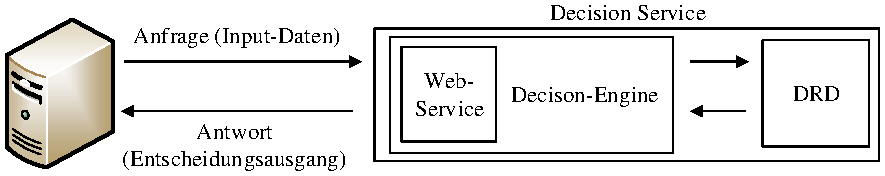
\includegraphics{images/decisionservice.pdf}
\caption{Überblick über die Komponenten bei der Implementierung eines DS.}
\label{fig:decisionservice}
\end{figure} 

Nach der theoretischen Beschreibung von DM und ML, werden einsetzbare Lösungen identifiziert,  die zur Implementierung des Prototypen verwendet werden können. Darüber hinaus wird dieses Kapitel darüber Aufschluss geben, wie diese zwei Grundlagenthemen zusammenhängen (siehe Abbildung \ref{fig:Grundlagenpic}).     

\begin{figure}[ht]
\centering
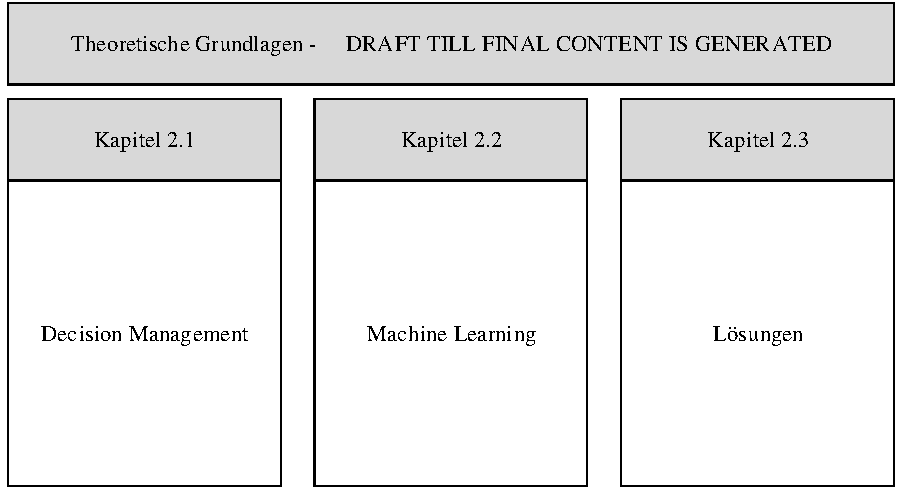
\includegraphics{images/grundlagentheo.pdf}
\caption{Die theoretischen Grundlagen im Überblick}
\label{fig:Grundlagenpic}
\end{figure}

Die Einzelnen Kapitel im Detail erklären .... (Erst möglich nachdem Sie geschrieben wurden)
\chapter{Konzeption}
\label{ch:Konzeption3}

Diese Kapitel beschreibt die Konzeptionsphase. Hierzu werden zu erst Anwendungsfälle definiert, um anschließend ein technisches Lösungskonzept auf Basis der Anwendungsfälle zu erarbeiten. 

\section{Definition von Anwendungsfällen}
\label{sec:Anwendungsfalle3}

\textbf{Kreditausfall-Erkennung:} Der zuerst gewählte Anwendungsfall ist das erkennen von Kreditausfällen. Ein Grund hierfür ist, dass diese Arbeit im Umfeld des Finanzsektors entsteht und somit sollen auch Anwendungsfälle aus diesem Bereich behandeln werden. Darüber hinaus besitzt das bestimmen des Kreditausfallrisikos einen sehr hohen Stellenwert innerhalb des Finanzsektors. Wie in Kapitel \ref{ch:Motivation1} bereits beschrieben, können Kredite die nicht zurückgezahlt werden zu hohen Verlusten bei Banken führen. Dies wiederum kann zu Finanzkrisen führen, die die komplette Weltbevölkerung in ihren Auswirkungen erreicht. Nichts desto trotz müssen auch die Interessen der Shareholder verfolgt werden. Daher soll ein Modell erlernt werden, dass ein Optimum zwischen Sicherheit und Gewinn gewährleistet. 

\textbf{Kreditkartenbetrugs-Erkennung:} Der Ansatz dieser Thesis soll anhand eines weiteren Anwendungsfall überprüft werden. Der zweite Anwendungsfall ist das Erkennen von betrügerischen Kreditkartentransaktionen. Studien wie \cite{FB11} zeigen, dass durch Kreditkartenbetrug in den Vereinigten Staaten im Jahr 2009, ein Schaden von 190 Milliarden Dollar entstanden ist. Ebenso zeigen Studien \cite[vgl. S. 24]{LE16}, dass im Jahr 2016 66\% aller Betrugsversuche erfolgreich sind. Aus diesem Grund wird untersucht werden, ob Machine Learning Verfahren Kreditkartenbetrug eindämmen können.   

\subsection{Erkennung von Kreditausfällen}
\label{subsec:Kreditausfallen3}

Ziel ist es Kreditanträge zu prüfen und die Ausfallwahrscheinlichkeit möglichst genau vorherzusagen. Hierzu müssen geeignete Daten verwendet werden um ein Modell zu erlernen, das die Vorhersagen treffen wird.

\subsection{Erkennung von Betrugsversuchen bei Kreditkartentransaktionen}
\label{subsec:Banktransaktionen3}

- Kurze Erläuterung von "'Fraud Detection"', sowie dessen Wichtigkeit

- Vorstellen des Datenschemas evtl. tabellarisch (Input und Output Data) 

- Vorstellen des Decision Tables

\section{Identifikation relevanter Themenfelder}
\label{subsec:Themenfelder3}

- Klären der Methodik des Prototyping um These zu beweisen

- Erläuterung des Prototypen und dessen Komponenten 
 
GRAFIK PROTOTYPE AT A GLANCE

\subsection{Basisdaten}
\label{subsec:Basisdaten3}

\textbf{Kreditausfall-Erkennung:} Nach ausgiebiger Recherche, konnten über ein Webportal der amerikanischen Hypothekenbank Fannie Mae, geeignete anonymisierte Kreditantragsdaten gefunden werden \cite{FM17}. Alle Datensätze entstammen Einfamilien-Immobilien-Dahrlehn. Die Kreditantragsdatensätze sind über Identifikationsnummern mit Performancedatensätzen verbunden, die das Zahlungsverhalten und weitere Informationen monatlich erfassen \cite{FM18}. Zum Download stehen die Acquisition- (Kreditantragsdaten) und die Performance-Datei (Performancedaten) bereit. Der erste Schritt zur Modellbildung ist die Aufbereitung der Lerndaten, diese bestehen aus Features und einem Label (vgl. \ref{sec:Machine_Learning2}).     
Als Features dienen die Kreditantragsdaten aus der Acquisition-Datei, wobei jeder Kreditantragsdatensatz mehrere Datensätze in der Performance-Datei besitzt. Aus den korrespondierenden Performancedatensätzen, muss für jeden Kreditantragsdatensatz das Label ermittelt werden. Die Kombination aus Features und Label bilden dann den Lerndatensatz. Abbildung \ref{fig:cleansing} soll den Prozess der Lerndatenerzeugung nochmals veranschaulichen.

\begin{figure}[ht]
\centering
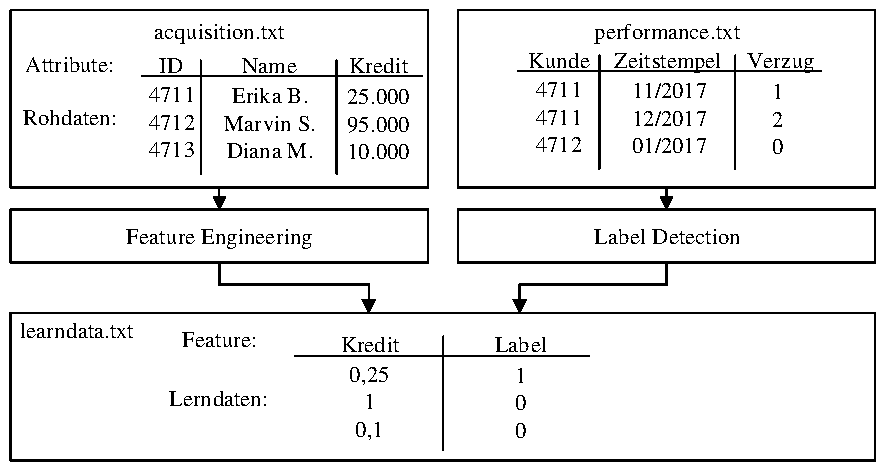
\includegraphics{images/cleansing.pdf}
\caption{Vorgehensweise bei der Erstellung des Lerndatensatzes.}
\label{fig:cleansing}
\end{figure}  

Jeder Datensatz aus der Performance-Datei stellt Informationen über Zahlungsverzüge bereit. Das Feature \textit{Current Loan Delinquency Status} beschreibt wie viele Monate der Kunde in Zahlungsverzug ist. Anhand der Identifikationsnummer wird der aktuellste Datensatz herausgesucht. Befindet sich der Kunde in Zahlungsverzug (Current Loan Delinquency Status > 0), wird dem Label der Wert 1 zu gewiesen. Liegt kein Zahlungsverzug vor wird der Wert 0 zu gewiesen. Darüber hinaus kann Current Loan Delinquency Status auch ''X'' annehmen, wenn der Zahlungsverzug unbekannt ist. Betroffenen Datensätze werden nicht zu Lerndatensätzen umgewandelt und werden übersprungen.  

\subsection{Lerndaten}
\label{subsec:Lerndaten3}

- Welche Daten werden benötigt um unser Neuronales Netz zu füttern.

- Erklärung des Erzeugungs-Algorithmus 

- Erklären von Feature Scaling

- Erklären von Labels

- Grafik mit Beispiel Datensätzen

\subsection{Evaluationsdaten}
\label{subsec:Evaluationsdaten3}

- Welche Daten werden benötigt um unser Neuronales Netz zu evaluieren.

- Erklärung des Erzeugungs-Algorithmus 

- Erklären von Feature Back Scaling

- Grafik mit Beispiel Datensätzen

\subsection{Decision-Engine}
\label{subsec:Engine3}

- Erklärung der theoretischen Funktionsweise der Decision Engine

- Erklärung des Stellenwerts innerhalb des Prototypen

\subsection{Neuronales-Netzwerk}
- Erklärung des Stellenwerts innerhalb des Prototypen 

- Funktionale Anforderungen: Lernen können sowie Datensatz evaluieren, sprich Output berechnen können

- Sollte leicht Anpassbar auf verschiedene Daten-Modelle bzw. UseCases sein 


\chapter{Implementierung}
- Dieses Kapitel beschreibt die Implementierung des (name?) Prototypen den wir zuvor konzipiert haben

\section{Datenschema}
- Ausgehend von den Zuvor in 3.2.1 und 3.2.2 beschriebenen Konzepten soll nun die Implementierung des Datenschemas beschrieben werden.

- H2-DB

- Sql-Script / Datenbankinhalt

- CSV Files bzw. deren Ersatz (in der Spätren Implementierung)

- Mit der erfolgreichen Implementierung der Datenschicht, haben wir nun eine Grundlage mit der wir später unser ML Verfahren sowie unsere Decison Engine füttern können.

\section{Decision-Engine}
- Implementierung Decision Engine 

- Nach Implementierung der Decision Engine muss nun das ML Verfahren implementiert werden, das unsere Entscheidungen verbessern soll

\section{Neuronales-Netzwerk}
- Implementierung nach unseren Anforderungen. 1. Lernen können und 2. Evaluieren können.  

- Erklären inwiefern DeepLearning4J leicht auf andere UseCases angewendet werden kann (Um das Kriterium der Allgemeingültigkeit zu erfüllen)

\section{Optimierung}
- Die Strukturen des NN wurden gesetzt. Nun müssen noch die Lernparameter bestimmt werden.

- Early Stopping using Best Model 

- Trial and Error

- Tabelle aus meiner PPT

- Evaluierungsdaten können auch gelernt werden 
\chapter{Analyse}
- Nach dem die Problemstellungen Px und Px gelöst wurden. 
- Kann die eigentliche Forschungsfrage dieser Thesis beantwortet werden

\section{Vorgehensweise}
- Hierzu sollen die Ergebnisse unseres Prototypen mit den Output-Werten der Decision Engine verglichen werden.

- Anhand der zwei Use Cases soll Verglichen werden, welches Verfahren (ML vs. DMN) statistisch bessere Ergebnisse liefert

\section{Erkennung von Kreditausfällen}
- Tabelle mit statistischen Werten 

\section{Erkennung von Betrugsversuchen bei Banktransaktionen}
- Tabelle mit statistischen Werten 

\section{Zusammenfassung der Ergebnisse}
- Tabelle mit statistischen Werten 
\chapter{Diskussion}

In diesem Kapitel werden die Ergebnisse der vorliegenden Arbeit diskutiert und bewertet

-> Wie aussagekräftig sind die Ergebnisse aus 5.1 bzw. 5.2

-> Was bedeutet das für die Forschungsfrage 

-> Welches Nutzen hat das für Anwender

-> Integration ACTICO Platform 

-> White Box <-> Blackbox
\chapter{Zusammenfassung und Ausblick}

- Diese Kapitel fasst die vorliegende Arbeit zusammen und soll darüber hinaus einen Ausblick geben wie der Prototyp weiter entwickelt werden könnte, bzw. wie ein Pilot-Projekt aussehen könnte
\cleardoublepage

\addcontentsline{toc}{chapter}{Literaturverzeichnis}
\printbibliography[title=Literaturverzeichnis]

\appendix
\appendix

\chapter{Anhang}

Lorem ipsum dolor sit amet, consetetur sadipscing elitr, sed diam nonumy eirmod tempor invidunt ut labore et dolore magna aliquyam erat, sed diam voluptua. At vero eos et accusam et justo duo dolores et ea rebum. Stet clita kasd gubergren, no sea takimata sanctus est Lorem ipsum dolor sit amet. Lorem ipsum dolor sit amet, consetetur sadipscing elitr, sed diam nonumy eirmod tempor invidunt ut labore et dolore magna aliquyam erat, sed diam voluptua. At vero eos et accusam et justo duo dolores et ea rebum. Stet clita kasd gubergren, no sea takimata sanctus est Lorem ipsum dolor sit amet.

Hier folgt Beispiel \ref{lst:xml} für Quellcode:

	\begin{lstlisting}[caption=XML-Konfiguration: settings.xml., label=lst:xml]
	<servers>
		<server>
			<id>xxx</id>
			<username>(Benutzername)</username>
			<password>(Passwort)</password>
		</server>
		<server>
			<id>yyy</id>
			<username>(Benutzername)</username>
			<password>(Passwort)</password>
		</server>
	</servers>
	\end{lstlisting}

\end{document}
